\documentclass[sigconf]{acmart}

\usepackage{booktabs}
\usepackage{amsmath}

\citestyle{acmauthoryear}
\setcitestyle{square}
\setcopyright{none}

\begin{document}

\title{Implementation of \textit{Rendering Fake Soft Shadows with Smoothies}}

\author{Sasha Volokh}
\email{sasha.volokh@gmail.com}

\begin{abstract}

In this report I will discuss various aspects of implementing the algorithm described in \textit{Rendering Fake Soft Shadows with Smoothies}. Specifically, I will discuss the tools used to accomplish the implementation, the places where implementing the algorithm was challenging given the design or limitations of these tools, provide a description of the implementation of each the stages of the algorithm, and finally analyze the results of the implementation.

\end{abstract}

\begin{teaserfigure}
  \centering
  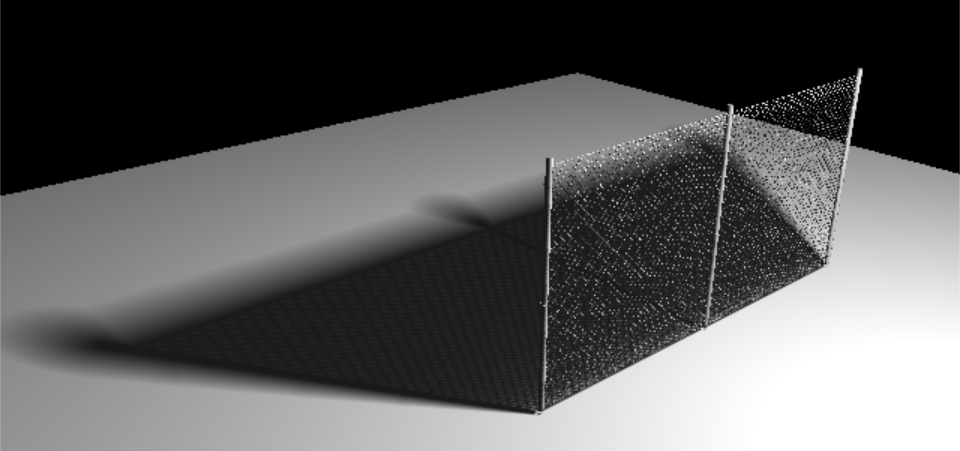
\includegraphics[width=6.0in]{reportfiles/teaser}
  \caption{Soft shadows produced by the implementation.}
\end{teaserfigure}

\maketitle

\section{Introduction}

The paper \textit{Rendering Fake Soft Shadows with Smoothies} describes an approach by which to construct fake soft shadows, called \textit{smoothies}, that resemble penumbrae and conceal aliasing along the edges of shadows in a traditional shadow map \cite{chan:smoothie:egsr2003}. In this report I will elaborate on the implementation process of this algorithm. For my implementation I took advantage of various features available in OpenGL 3+, such as Vertex Arrays and Framebuffer Objects, version 1.5 of the \textit{OpenGL Shading Language (GLSL)}, and the \textit{OpenGL Mathematics (GLM)} library for graphics-specific matrix math. The implementation consists of a one-time initialization phase, during which models are loaded and data structures for the efficient computation of smoothies are prepared, a lighting calculation phase, during which for all scene lights that are uninitialized or dirtied smoothie geometry is constructed, shadow maps are rendered, and smoothie buffers are rendered, and finally a scene rendering phase, during which diffuse lighting and shadowing is performed through the use of the light shadow maps and smoothie buffers.

\section{Initialization Phase}

During the initialization phase, models are loaded and data structures are prepared for each model to aid in the future computation of smoothie geometry.

\subsection{Model Loading}

For each model three datasets are loaded: vertices, normals, and indices. Each vertex and normal is a 3-tuple of floats specifying the x, y, and z values. Every 3 consecutive indices specify a triangle, and an index refers to a vertex and its normal. For some arbitrary meshes computing the normals can be ambiguous, and furthermore modelling tools such as \textit{Blender} can provide interpolated normals that enable smooth diffuse shading, so thus it is better to rely on provided normal data.

\subsection{Preparation For Smoothies}

When constructing smoothie geometry, edges are considered silhouette edges if one of their triangles faces away from the light, and the other faces towards the light. My algorithm uses the same brute-force algorithm described in the paper for computing silhouette edges, where I traverse all edges and perform the test for each edge. For this algorithm it is efficient to have a mapping from edges to triangles, and thus for each model I compute and store this mapping in C++'s \texttt{std::map}, an implementation of a red-black tree.

\section{Lighting Calculation Phase}

In the lighting calculation phase, I construct smoothie geometry, render shadow maps, and render smoothie buffers.

\subsection{Constructing Smoothie Geometry}

\begin{figure}[t]
    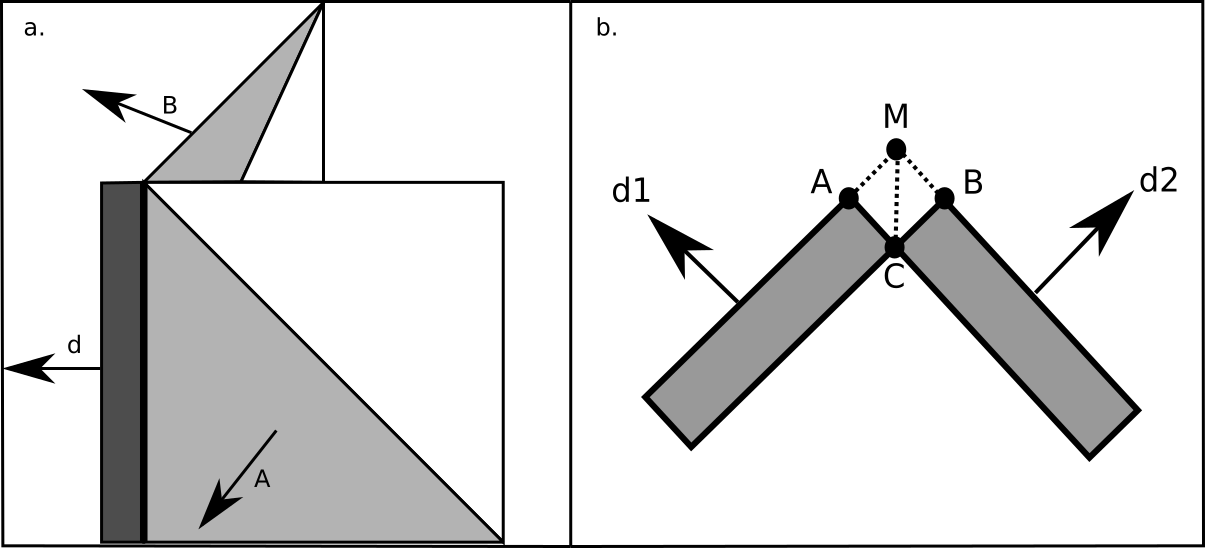
\includegraphics[width=\linewidth]{reportfiles/smoothie-construction}
    \caption{(a) demonstrates extruding a silhouette edge to form a smoothie edge. Normals \textbf{A} and \textbf{B} are averaged in screen-space to determine whether \textbf{d} should be facing left or right. (b) demonstrates creating a silhouette corner in screen-space by intersecting the lines created by point \textbf{A} and normal \textbf{d1} and point \textbf{B} and normal \textbf{d2}.}
    \label{fig:smoothie-construction}
\end{figure}

At the start of the light calculation phase, for each model, I use the edge-to-triangle mapping to compute a list of all silhouette edges. Then, I construct the smoothie edges and corners in screen-space. As shown in diagram (a) of figure \ref{fig:smoothie-construction}, to determine the direction in which to extrude the silhouette edge, I average the normals $\vec{A}$ and $\vec{B}$ of the adjacent triangles in screen-space to obtain a vector whose dot product with the extrusion vector should be positive. $\vec{d}$ is first computed by rotating the silhouette edge {90\textdegree} in screen-space. If the dot product of $\vec{d}$ and that vector is negative, then I flip the direction of $\vec{d}$.

For corners, as demonstrated in diagram (b) of figure \ref{fig:smoothie-construction}, I intersect the line created by the two smoothie edges to obtain the two triangles of the corner. For complex meshes it is also possible that in screen-space $A$ and $B$ are at the same position. For this case I omit the construction of the corner.

I store each smoothie edge as two triangles in a smoothie edge vertex buffer, with each vertex entry containing the coordinate in screen-space and the linear alpha value. The vertex on the silhouette edge receives an alpha of 0, and the vertex on the extruded edge receives an alpha of 1. The alpha correction with respect to the smoothie shadow receiver is done later in the fragment shading stage during smoothie rendering.

I store each smoothie corner as two triangles in its own vertex buffer. For this buffer, each vertex entry contains the coordinates in screen-space, as well as the origin point $C$ to be used later in the fragment shading stage for creating a circular alpha transition around the origin. 

With the smoothie edge and corner buffers prepared, the model's smoothies are ready for rendering.

\subsection{Rendering Shadow Maps}

\begin{figure}[t]
    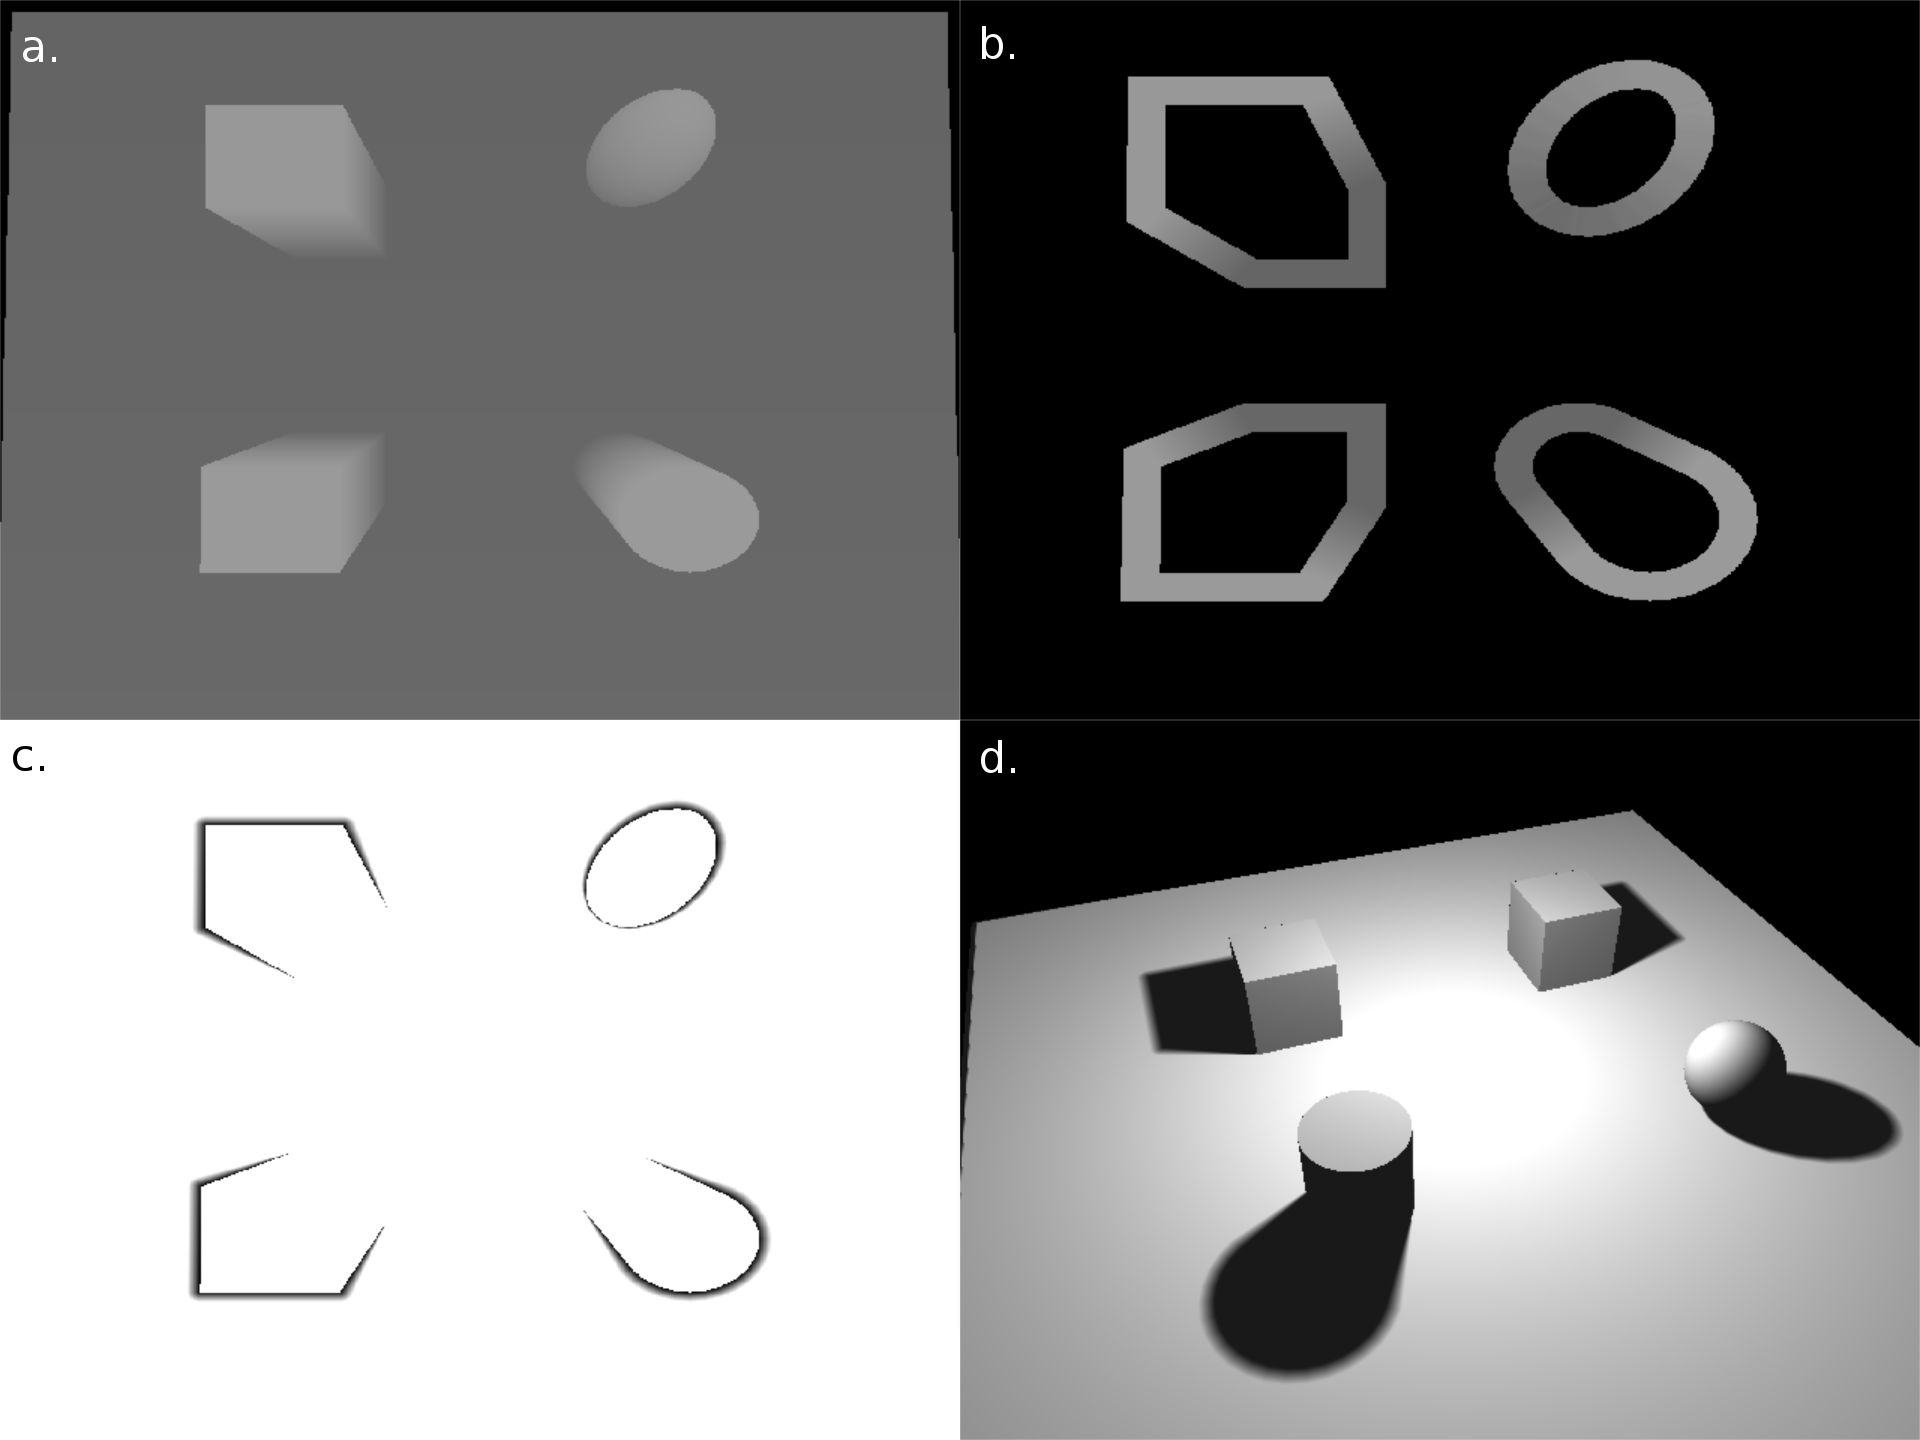
\includegraphics[width=\linewidth]{reportfiles/render-phases}
    \caption{(a): The shadow map rendered for the scene from the scene's light source. (b): The smoothie buffer's depth rendered for the scene from the scene's light source. (c): The smoothie buffer's alpha rendered for the scene from the scene's light source. (d): The scene rendered with diffuse shading and resulting shadows.}
    \label{fig:render-phases}
\end{figure}

Rendering the smoothie buffers requires the shadow map to be present, as the smoothie buffer rendering phase needs to know the depth of the smoothie shadow receiver. So, before I render the smoothie buffer, I render the shadow map. The standard OpenGL depth buffer cannot be used for this, however, as linear depth values are necessary for computing the alpha correction. To handle this I write linear depth values from the fragment shader to a 32-bit float texture and then use OpenGL's minimum blending to get the closest depth values. Diagram (a) in figure \ref{fig:render-phases} displays an example of the contents of the shadow map.

\subsection{Rendering Smoothie Buffers}

The smoothie buffer contains two components: a depth component, which stores the depth value of the smoothie edges and corners, and an alpha component, which specifies how much shadow a region of a smoothie should produce. In my implementation I used two separate buffers to store the depth and the alpha.

\subsection{Smoothie Depth Buffer}

The smoothie depth buffer is rendered by simply taking the depth values given by the vertex shader and interpolating them (this is handled automatically by the rasterization stage). Diagram (b) in figure \ref{fig:render-phases} demonstrates the contents of a smoothie depth buffer.

\subsection{Smoothie Alpha Buffer}

For rendering the smoothie alpha buffer, in the fragment shader, I obtain $\alpha$, then use \[ \alpha' = \frac{\alpha}{1 - b/r}  \] as given by the paper to obtain the corrected alpha, where $b$ is the linear depth of the blocker, and $r$ is the linear depth of the receiver. I then clamp $\alpha'$ in range $[0, 1]$. To obtain $b$, I use the interpolated depth of the smoothie triangle in camera space provided by the vertex shader, and to obtain $r$ I perform a lookup inside the linear shadow map constructed earlier. One special case that needs to be considered here is when $b \approx r$. This case causes $1 - b/r$ to approach zero, which can be problematic if $\alpha \approx 0$. To handle this case, if $1 - b/r \approx 0$, I set $\alpha' = 1$.

For smoothie edges, $\alpha$ comes from the interpolation of alphas given by the vertex shader. For smoothie corners, $\alpha$ comes from \[ \alpha = \frac{|\vec{v} - \vec{p}|}{t} \] as given by the paper, where $\vec{v}$ is the origin (that was stored as a vertex attribute during smoothie geometry construction and then provided to the fragment shader by the vertex shader), $\vec{p}$ is the current position in the fragment, and $t$ is the smoothie size.

Diagram (c) of figure \ref{fig:render-phases} demonstrates the contents of a smoothie alpha buffer.

\section{Scene Rendering}

With the shadow map and smoothie buffer available, the scene can now be rendered. At the scene rendering stage, the fragment shader implements diffuse shading and shadowing. For diffuse shading I use a phong shading approach: given the interpolated surface normal $\vec{n}$ and a computed direction to the light $\vec{l}$, I compute the diffuse factor as $\mathit{diffuse} = \mathit{max}(0, \vec{n} \cdot \vec{l})$. 

For computing the shadow factor $\mathit{shadow}$ (0 for fully shadowed, 1 for fully visible), I use the shadow map view-projection matrix $M_\mathit{vp}$ to compute screen-space coordinate $\vec{p_s}$ from world-space coordinate $\vec{p_w}$ with \[ \vec{p_s} = M_\mathit{vp} \cdot \vec{p_w} \] Then, I perform a lookup into the shadow map to obtain shadow map depth $d_s$, and a lookup into the smoothie depth buffer to obtain smoothie depth $d_m$. For given linear fragment depth $d$, \[ 
\mathit{shadow} = \begin{cases}
    0 & d > d_s \\
    \alpha' & d > d_m \\
    1 & \mathit{otherwise}
\end{cases}
\] where $\alpha'$ is the corrected alpha from the smoothie alpha buffer. 

I perform this lookup on the four nearest texels in the shadow maps and smoothie buffers, and then perform a weighted average of the result to obtain an interpolated shadow. 

Finally, I calculate the fragment color as \[ \mathit{clamp}(\mathit{ambient} + \mathit{shadow} * \mathit{diffuse}, 0, 1) \]

\section{Performance Analysis}

With smoothies, the two main bottlenecks are in the smoothie geometry construction phase, where silhouette edges must be identified, and the smoothie rendering phase, where an additional rendering pass must be performed after the shadow map render to produce the smoothie buffers.

\subsection{Smoothie Geometry Construction Performance}

\begin{figure}[t]
    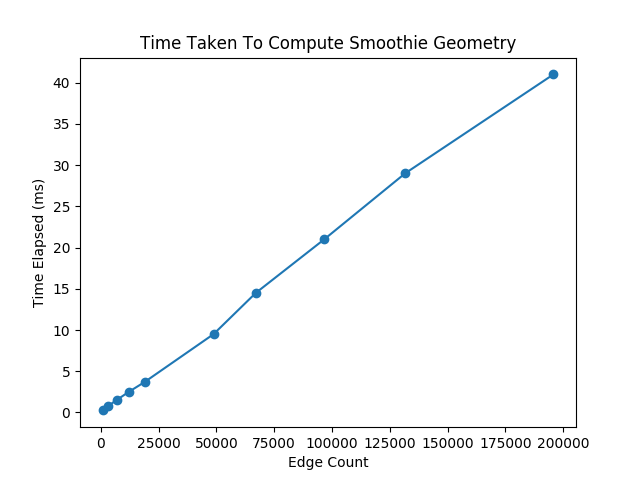
\includegraphics[width=\linewidth]{reportfiles/time-taken-to-compute-smoothie-geometry}
    \caption{The time taken to identify silhouette edges and construct smoothie geometry.}
    \label{fig:time-taken-to-compute-smoothie-geometry}
\end{figure}

As mentioned earlier, for identifying silhouette edges I use the brute-force algorithm, where I traverse each edge and check its adjacent triangles to see if one faces the light source and the other faces away. As expected, in figure \ref{fig:time-taken-to-compute-smoothie-geometry}, we see a linear increase in the time taken to construct smoothie geometry.

Whenever the light source changes, smoothie geometry must be reconstructed and subsequently silhouettes must be recomputed. Thus for real-world applications such as in games, where high polygon-count models are to be expected and light sources can be highly dynamic, an efficient algorithm for silhouette identification is critical. There exists a more efficient tree-based algorithm for static models to improve on this \cite{chan:smoothie:egsr2003}, however it was not part of this implementation.

\subsection{Smoothie Buffer Render Performance}

\begin{figure}[t]
    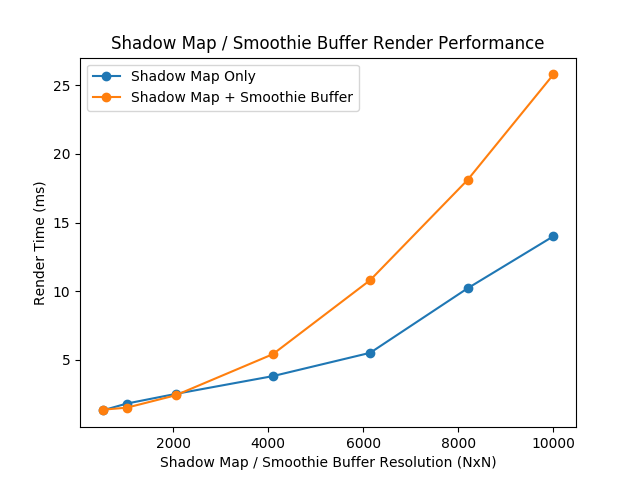
\includegraphics[width=\linewidth]{reportfiles/sm-smoothie-buffer-render-performance}
    \caption{For a scene with 130,000 edges, a comparison of the time taken to render the shadow map alone versus the shadow map and the smoothie buffers. The smoothie buffers are rendered with the smoothie geometry already given (i.e. the time taken to compute the smoothie geometry on the CPU is not counted here).}
    \label{fig:sm-smoothie-buffer-render-performance}
\end{figure}

The smoothie buffer rendering pass is another spot that introduces overhead. In figure \ref{fig:sm-smoothie-buffer-render-performance} we can see that for very high-resolution shadow maps the difference is significant, but not so much for shadow maps below the 4096x4096 mark. The overhead is small because unlike in the shadow map render, where each triangle in the scene must be rendered, only geometry related to the silhouettes is rendered. However, there are still texture lookups performed for each smoothie fragment and a non-trivial vector magnitude computation in the corners for computing the rounded alpha, so there is still some expense in rendering these triangles.

\section{Visual Analysis}

To analyze the effectiveness of smoothies I will consider a simple closed mesh (a cylinder) as did the paper, and then I will further discuss the effectiveness of the algorithm in a complex mesh with many holes (a fence). Finally, I will touch on the algorithm's handling of overlapping figures.

\subsection{Simple Mesh}

\begin{figure}[t]
    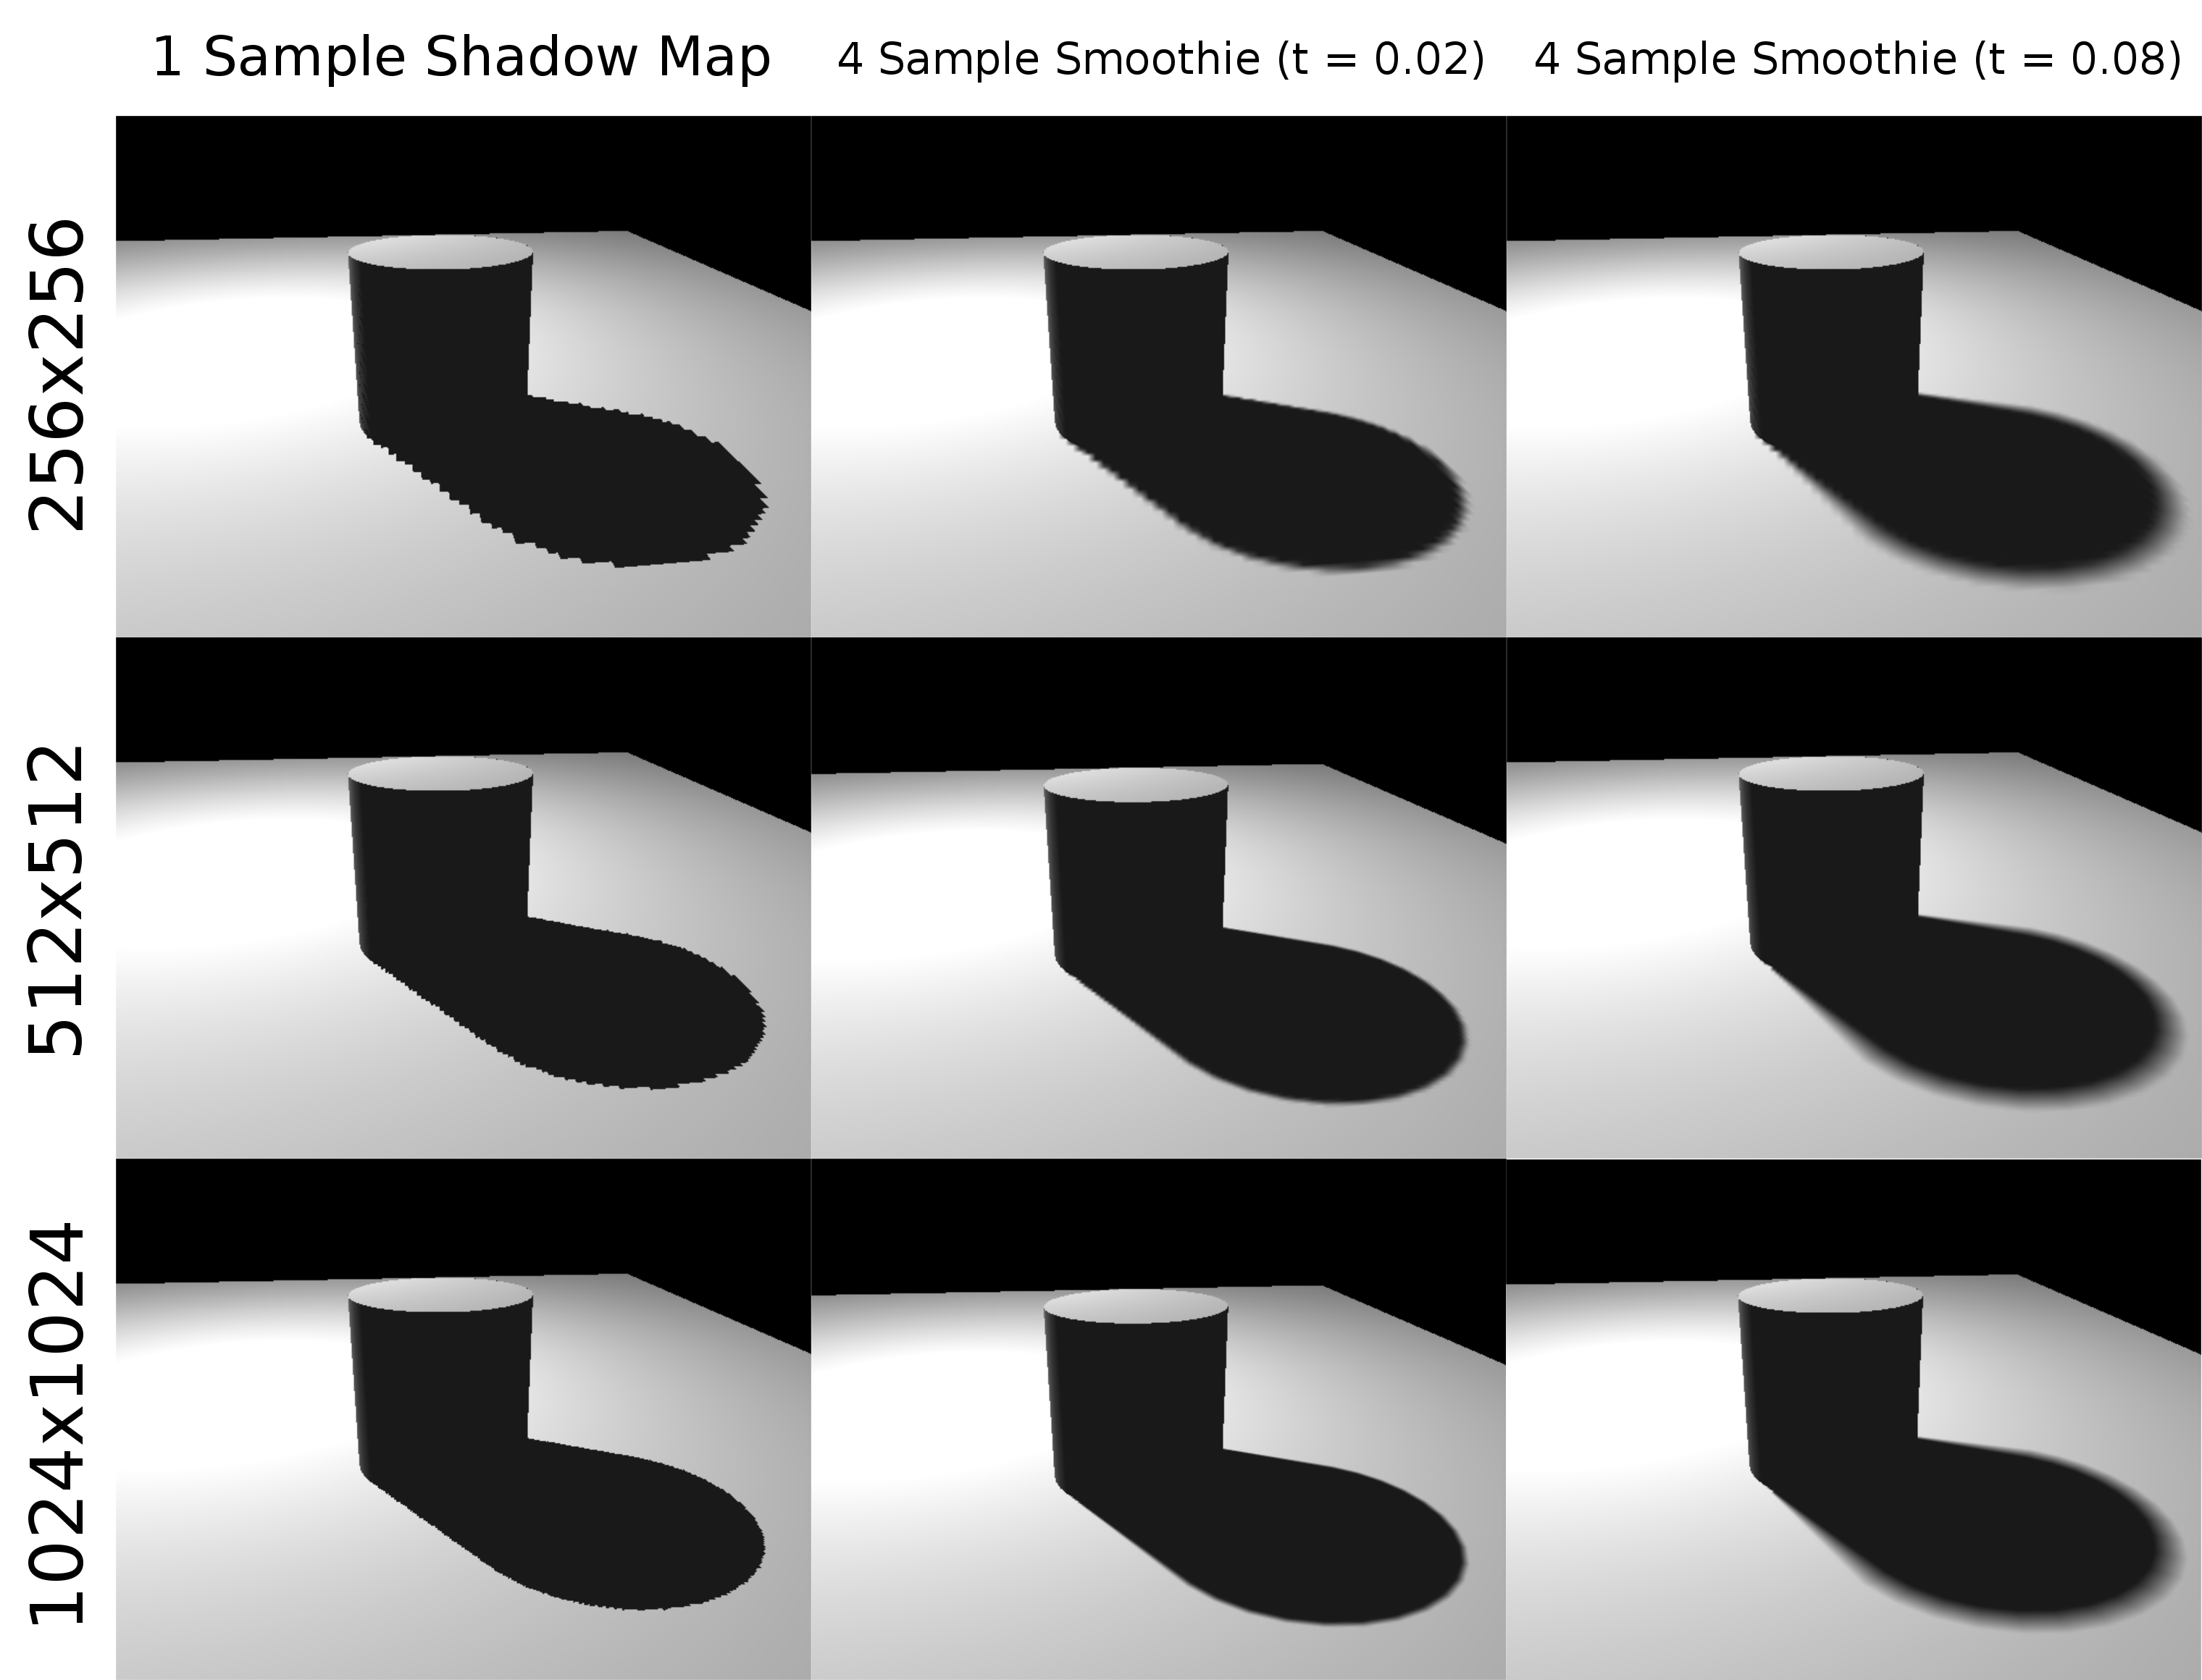
\includegraphics[width=\linewidth]{reportfiles/simple-visuals}
    \caption{Comparison of the different shadows produced for a simple closed mesh when varying shadow map / smoothie buffer resolutions and shadowing methods.}
    \label{fig:simple-visuals}
\end{figure}

In figure \ref{fig:simple-visuals} we can see a comparison of different shadowing approaches for a simple cylinder. Even at high resolutions shadowing with single-sampling of the shadow map has very visible aliasing, which is concealed effectively by the smoothies. For the low-resolution buffer at 256x256, a thin smoothie does not conceal all aliasing, however a thicker one performs better.

\subsection{Complex Mesh}

\begin{figure}[t]
    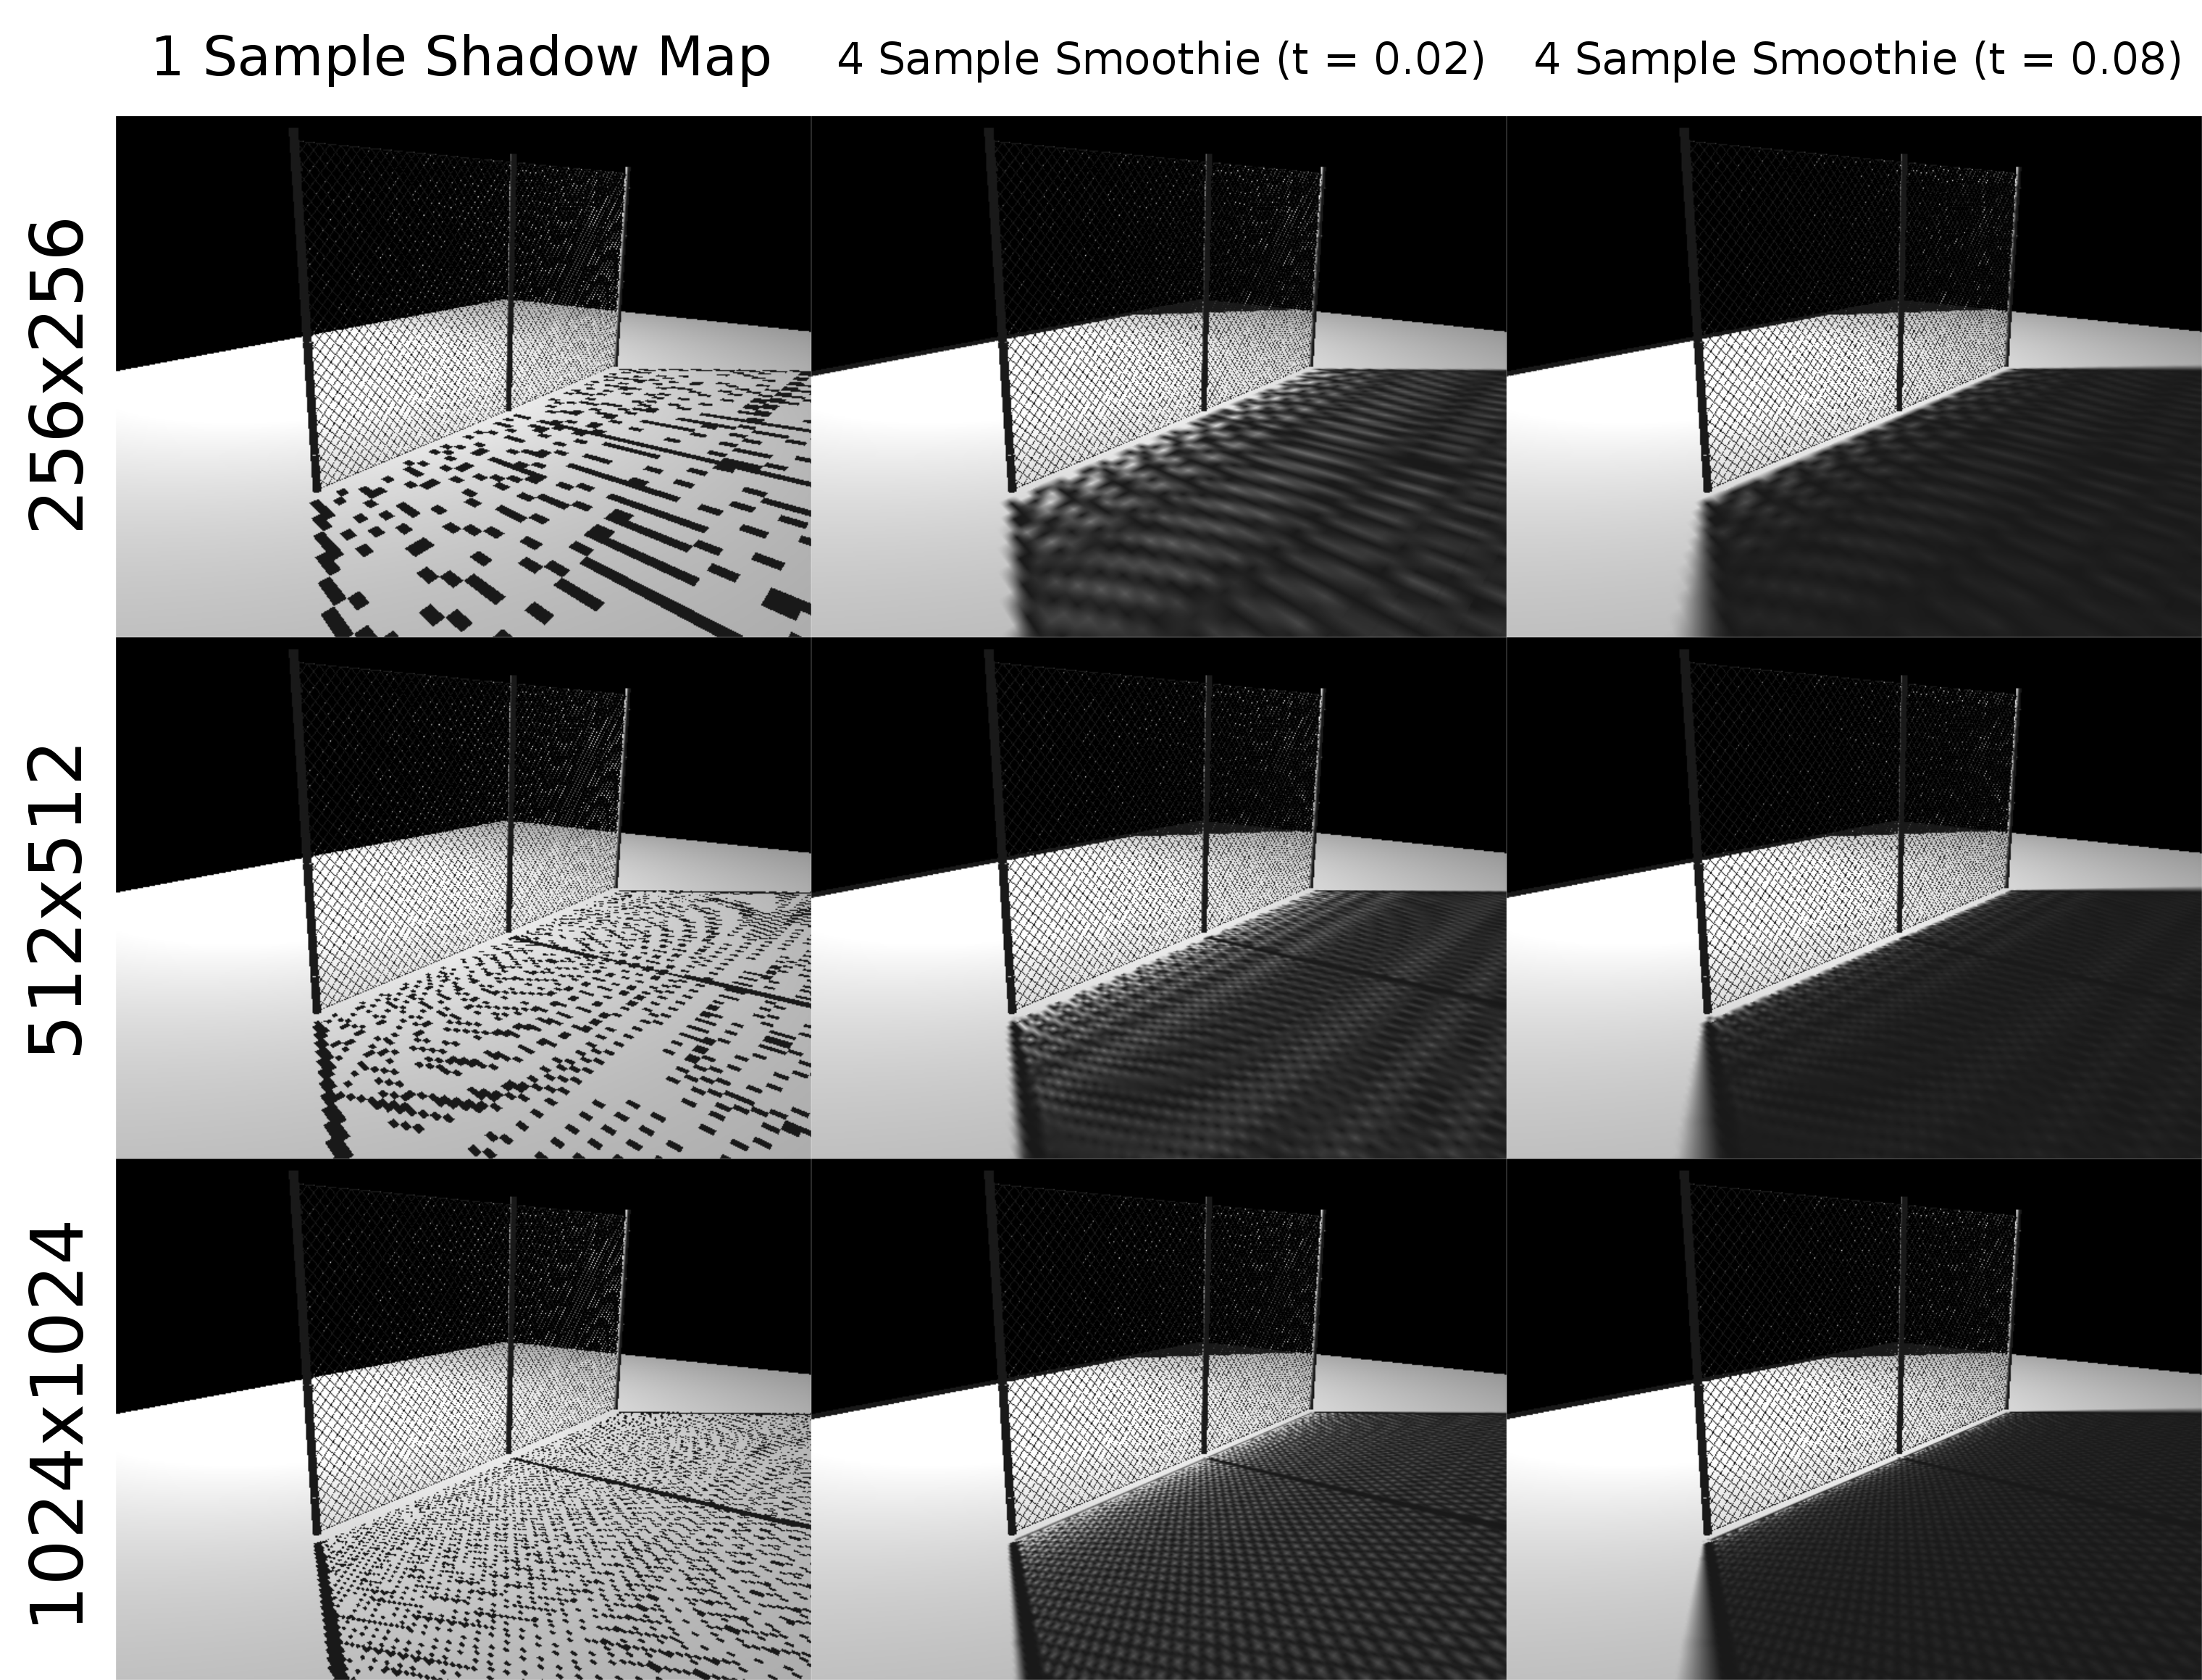
\includegraphics[width=\linewidth]{reportfiles/complex-visuals}
    \caption{Comparison of the different shadows produced for a complex mesh with holes when varying shadow map / smoothie buffer resolutions and shadowing methods.}
    \label{fig:complex-visuals}
\end{figure}

In figure \ref{fig:complex-visuals} we can see a comparison for a fence. For the lowest resolution of 256x256, none of the options look very appealing, but the smoothies clearly provide a more complete shape for the shadow. At 1024x1024, whereas single-sampling the shadow map still provides poor results, we can see a more complete shadow for the fence with thinner smoothies. Evidently, for meshes with small openings it is better to use a thinner smoothie, as a thicker one creates a shadow that is too dark.

\section{Other Observations}

\begin{figure}[ht]
    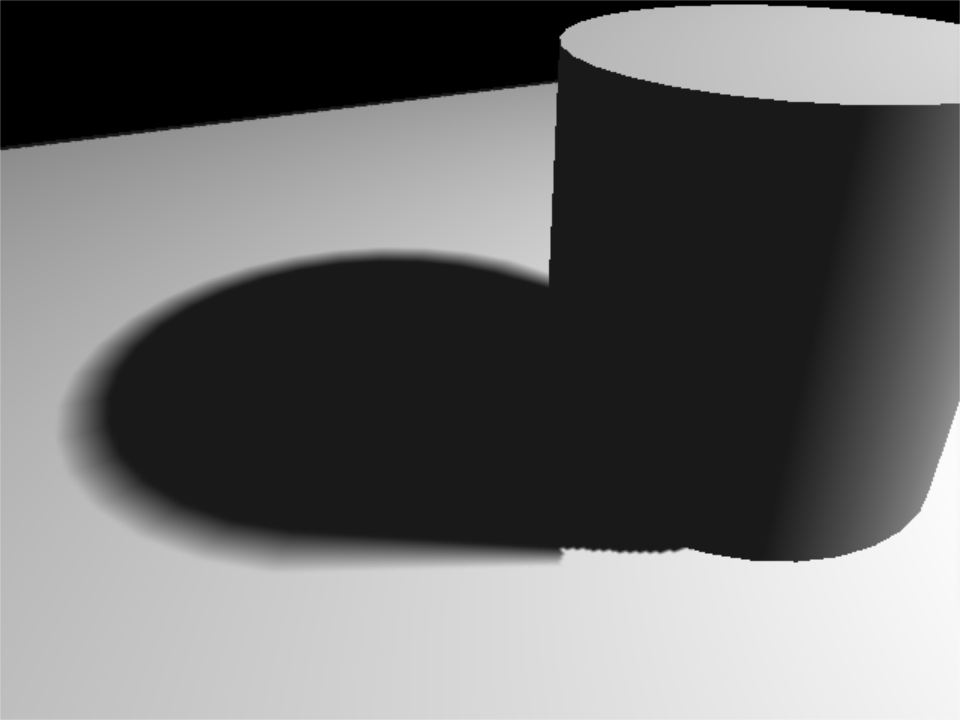
\includegraphics[width=\linewidth]{reportfiles/smoothie-discontinuity-due-to-bias}
    \caption{Smoothie discontinuity due to an over-sized depth bias.}
    \label{fig:smoothie-discontinuity}
\end{figure}

Various other items of note appeared during the implementation process. When using an over-sized depth bias that results in noticeable ``Peter panning'' of shadow map shadows, the difference in depth between the smoothies and shadow map also causes a discontinuity in the soft shadow edges, as demonstrated in figure \ref{fig:smoothie-discontinuity}. 

When experimenting with dynamic lighting (lighting that changes each frame), I also noticed that for low polygon-count models, where silhouette edges can change more harshly between frames, thick smoothies have a very noticeable ``snapping'' effect in the scene. This effect does not appear with high polygon-count models, where silhouette edges would be closer together between frames.

\section{Conclusion}

In conclusion, my implementation has demonstrated how smoothies are a cost-effective way to create fake soft shadows that also conceal shadow map aliasing. The primary bottleneck in my implementation is in the identification of silhouettes, for which I currently use a brute-force algorithm, however this bottleneck is only relevant when the light source is dynamic. After the identification of silhouettes however, the smoothie buffer rendering pass does not introduce much overhead for common shadow map resolutions, and is well worth it for the improvement seen across all shadow map resolutions.
    
\bibliographystyle{ACM-Reference-Format}
\bibliography{report}
\end{document}
